\documentclass[12pt, letterpaper]{article}

\usepackage{float}
\usepackage{amsmath}
\usepackage{hyperref}

\usepackage{tikz}
\usepackage{caption}
\usetikzlibrary{matrix, positioning}
\tikzset{bullet/.style={circle,fill,inner sep=2pt}}

\usepackage{graphicx}
\graphicspath{ {./images/} }

\usepackage{geometry}
\geometry{margin=1in}

\begin{document}

\title{Binomial Pricing Model \\
\large Probability and Inference}
\author{Charlie Liu}
\date{\today}
\maketitle

\section*{Introduction}

In finance and economics, the asset market is a blanket term that covers all the various underlying markets that involve the exchange of financial assets.
The stock market is one popular example of an underlying market where buyers and sellers can exchange assets in the form of stocks/shares (ownership) of a company.
Other notable markets include the bond market where fixed-income assets like corporate bonds are exchanged, and the derivatives market where contracts between two consenting parties are exchanged.
The different types of markets can be accessed depends on the features provided by the service or brokerage used.


Since the goal when exchanging financial assets is to obtain profit or minimize loses, one must account for the valuation of the asset being exchanged.
The valuation of an asset is based on the future expected cash flow (CHAPTER5PDF) and is especially important when exchanging assets because pricing is typically determined by the seller and influenced by the buyers.
It is important to note here that because asset valuation is based on future expected cash flow, any calculated valuation such as intrinsic (justified) valuation is considered theoretical.
This is why quantitative analysis is heavily used in asset valuation as the various mathematical models and technicals/fundamentals are used to estimate the valution of an asset.
For stocks and bonds, there are various ways to obtain the intrinsic value through different mathematical models; some of which are listed here: (https://xplaind.com/746919/stock-valuation).


For financial derivatives, valuation is a lot harder to calculate because they are essentially contracts that \_derive\_ their value from the performance of the underlying entity %(https://en.wikipedia.org/wiki/Derivative_(finance)).
Since asset valuation is already difficult to calculate and are theoretical, financial derivatives are like an extra layer of theoretical valuation on top of theoretical valuation.
One notable financial derivative is the option contract. 
Option contracts gives the buyer the right to "exercise" the contract which means the contract holder can either buy or sell the underlying entity (usually stock) at a fixed price once a certain price threshold called the strike price is met.
In order to profit from exercising the option, the amount generated from buying or selling at the strike price must cover the cost of the option.
All option contracts come with an expiration time.
If the strike price condition is not met for the option contract, then the contract is considered worthless and will "expire" which results in a loss based on the amount paid for on the option contract.
This "expiration" is also called "maturity".
An option contract to buy the underlying entity is called a call and an option contract to sell the underlying entity is called a put.
One may buy a call or put option on the market and then sell that same option contract on the market.

The benefit of options is the leveraged returns and its main disadvantage is the leveraged risk.
The price of an option contract is essentially the premium fee paid per share times the number of shares listed in the contract (which is typically 100 shares).
This means if an option contract average bid-ask price was \$0.42/share, then the actual amount needed to purchase the option would be \$0.42 x 100= \$42.00.
This also means that if the average bid-ask spread of the option increases from \$0.42/share to \$0.80/share, then the option can be resold on the market for a \$0.38/share or \$38.00 profit, which is a \~90.47\% increase from the initial investment.
This effect also works in the opposite direction, where if the average bid-ask price of the option decreased to \$0.08, then there would be a loss of \~80.95\% from the initial investment.

Various factors can have different effects on the valuation of the option contract. 

The famous mathematical model called the Black-Scholes Model developed by Fischer Black, Myron Scholes, and Robert C. Merton was able to give a theoretical valuation of European-style options (https://en.wikipedia.org/wiki/Black-Scholes\_model).
There is emphasis on "European-style" options in this case because the Black-Scholes model (by itself) is only accurate on the European-style options.
European-style options only allow exercise on expiration/maturity, while American-style options allow the holder to exercise before expiration.
This early exercise of the American-style options makes it difficult to find the optimal time to exercise the option for maximum gains (https://en.wikipedia.org/wiki/Black-Scholes\_model) as the Black-Scholes model cannot account for the various outcomes before expiration. 

The Binomial options pricing model, developed in 1979, overcame this limitation for the American-style options (LIST CREDITORS).
Its feature of generating "nodes" that represent different possible outcomes over a period of time allows for better insight into the optimal stop.

Some more commentary is provided in the "Commentary Section" below to compare both models.

\pagebreak

\section*{Methods}

The binomial options pricing model aims to find the valuation of the chosen option at discrete times based on various inputs given.
It achieves this by generating a binomial decision tree where each node represents the valuation of the option at a certain point in time.
This binomial tree is essentially a lattice of Bernoulli processes in which each path represents a Bernoulli process because at each [non end/start] node there are two directional outcomes of the stock: up or down.
This also means that the probabilities for up and down movement are p and 1-p respectively where 0 $\leq$ p $\leq$ 1.

\begin{figure}[H]
  \centering
  \begin{tikzpicture}[>=stealth, sloped, baseline]
    \matrix (tree) [%
      matrix of nodes,
      minimum size=1cm,
      column sep=2cm,
      row sep=1cm, nodes={text width=5em}
      	]
      {
  		  t=0 & t=1 & t=2 \\
  
            &  &  ${}$ \\
  
        	&  {}  &\\
  
        ${S}_0$  &  &  ${}$\\
  
        	&  {}  &\\
  
            &  &  ${}$ \\
      };
      \node[bullet, left=0mm of tree-2-3.west, label=above:${u^2S}$, label=below:${V_{2,n}}$](b-2-3){};
      \node[bullet, left=0mm of tree-3-2.west, label=above:${uS}$, label=below:${V_{1,n}}$](b-3-2){};
      \node[bullet, right=7mm of tree-4-1.west](b-4-1){};
      \node[bullet, left=0mm of tree-4-3.west, label=above:${udS}$, label=below:${V_{2,n}}$](b-4-3){};
      \node[bullet, left=0mm of tree-5-2.west, label=above:${dS}$, label=below:${V_{1,n}}$](b-5-2){};
      \node[bullet, left=0mm of tree-6-3.west, label=above:${u^2S}$, label=below:${V_{2,n}}$](b-6-3){};
      \draw[->] (b-4-1) -- (b-3-2) node [midway,above] {$p$};
      \draw[->] (b-4-1) -- (b-5-2) node [midway,below] {$(1-p)$};
      
  		\draw[->] (b-3-2) -- (b-2-3) node [midway,above] {$p$};
      \draw[->] (b-3-2) -- (b-4-3) node [midway,below] {$(1-p)$};
  
  		\draw[->] (b-5-2) -- (b-4-3) node [midway,above] {$p$};
      \draw[->] (b-5-2) -- (b-6-3) node [midway,below] {$(1-p)$};
  \end{tikzpicture}
  \caption{A generic binomial options pricing lattice with 2 periods}
\end{figure}


There are two ways to obtain the valuation of the option using this model.
One way is thorugh a method called "delta-hedging" and the other is to use the probabilities for each node path.
The novel feature of this model is that option valuation can be achieved without the need of probabilities through delta-hedging.
If obtaining the valuation through probabilities, the expected return would be based on the probabilities inputed, but the problem is that the true probabilities are unknown.
This same feature is what made Black-Scholes famous in that the true probabilities and expected returns were uneccessary to obtain the valuation of the given option contract. (https://www.youtube.com/watch?v=PZrmOh2nZus)

For this paper, only the probabilities method will be used to obtain the valuation of the given option. 

The process to evaluate the given option is described as a three step process: %(https://en.wikipedia.org/wiki/Binomial_options_pricing_model)

1. Price tree generation
2. Calculation of option value at each final node
3. Sequential calculation of the option value at each preceding node

To best describe this method, it's best to have an example.

Here are some variables that need to be established:

Let ${\textit{\textbf{(S)}}}$: \textit{\textbf{Stock Price}} = 100

Let ${\textit{\textbf{(X)}}}$: \textit{\textbf{Strike Price}} = 120

Let ${\textit{\textbf{(r)}}}$: \textit{\textbf{Risk-Free Interest Rate}} = 0.09\%

Let ${\textit{\textbf{(u)}}}$: \textit{\textbf{Up Factor}} = 1.25

Let ${\textit{\textbf{(d)}}}$: \textit{\textbf{Down Factor}} = 1/u = 1/1.25 = 0.80

Let ${\textit{\textbf{(T)}}}$: \textit{\textbf{Time (year(s))}}  = 1

Let ${\textit{\textbf{(t)}}}$: \textit{\textbf{Time Periods}}  = 2 

\pagebreak
\subsection*{1. Price Tree Generation}
\subsubsection*{Establishing Movement Factors}
"u": the fixed factor in which the price of the underlying stock increases by.
"d": the fixed factor in which the price of the underlying stock decrease by.

It is suggested that in the original 1979 CRR paper that:
\begin{equation*}
  \setlength{\jot}{10pt}
  \begin{split}
    u
    & = e^{\sigma\sqrt{t/n}}
    \\
    d
    & = e^{-\sigma\sqrt{t/n}} = \frac{1}{u}
  \end{split}
\end{equation*}

In which:
${\sigma}$ represents the volatility (standard deviation) of the stock price (add footnote about this) %https://en.wikipedia.org/wiki/Volatility_(finance)
${t/n}$ represents the time where "t" is the fixed length of time left to expiration and "n" is the number of periods left before expiration

One neat thing about these formulas is that the stock price at a certain time period ${n}$ can be calculated with this formula:
\begin{equation*}
  {S}_n = {S}_0 \cdot {u}^{N_u-N_d}
\end{equation*}

Since nodes with paths ${u > d}$:
\begin{equation*}
  \setlength{\jot}{10pt}
  \begin{split}
    {S}_n
    & = {S}_0 \cdot {u}^{N_u-N_d}
    \\
    & = {S}_0 \cdot {u}^n
  \end{split}
\end{equation*}

Nodes with paths ${u < d}$:
\begin{equation*}
  \setlength{\jot}{10pt}
  \begin{split}
    {S}_n
    & = {S}_0 \cdot {u}^{N_u-N_d}
    \\
    & = {S}_0 \cdot {1/u^n}
    \\
    & = {S}_0 \cdot ({1/u})^n
    \\
    & = {S}_0 \cdot {d^n}
  \end{split}
\end{equation*}

And nodes with paths ${u = d}$:
\begin{equation*}
  \setlength{\jot}{10pt}
  \begin{split}
    {S}_n
    & = {S}_0 \cdot {u}^{N_u-N_d}
    \\
    & = {S}_0 \cdot {u^0}
    \\
    & = {S}_0 \cdot 1
    \\
    & = {S}_0
  \end{split}
\end{equation*}


And this in-turn is derived from the continous compouding formula: %https://en.wikipedia.org/wiki/Compound_interest https://en.wikipedia.org/wiki/Characterizations_of_the_exponential_function
${P(t)} = {P}_{0}e^{rt}$

Because the value at each consecutive node is essentially the initial value of the stock compounded by the stock's movement factor at a certain period.

* Note the following is commentary of an assumption based on the research done.

This compound rate: ${\sigma\sqrt{2/\pi}}$ for call and ${-\sigma\sqrt{t/n}}$ bears a resemblance and is probably derived from the mean absolute deviation (MAD) of the normal distribution:
\begin{equation*}
  MAD = \sigma\sqrt{2/\pi}
\end{equation*}

According wikipedia on average/mean absolute deviation, the "MAD is the average of the absolute deviation from a central point".
Which in this context means that "u" would be componding of the absolute deviation of the underlying stock.
%(Source: https://en.wikipedia.org/wiki/Average_absolute_deviation )

\subsubsection*{Risk-free interest rate}

"r": the risk-free interest rate %[insert footnote here about what it is]
This value represents the safest interest one would get if they were to put the money in that asset.
The most common risk-free interest used is the U.S Treasury bond yields as the bonds are considered the safest (the risk is so low that its negligible) assets to obtain interest.

For simplicity, this paper will use 0.09\% from the current 6-month U.S Treasury bill as the risk-free interest rate for calculations.
%(According to https://www.treasury.gov/resource-center/data-chart-center/interest-rates/Pages/TextView.aspx?data=yield for Nov 25, 2020)

\subsubsection*{Generated Tree}
Given the variables for this example, the tree with stock price estimates is generated below:
\begin{figure}[H]
  \centering
  \begin{tikzpicture}[>=stealth, sloped, baseline]
    \matrix (tree) [%
      matrix of nodes,
      minimum size=1cm,
      column sep=2cm,
      row sep=1cm, nodes={text width=5em}
      	]
      {
  		  t=0 & t=1 & t=2 \\
  
  					&  &  ${}$ \\
  
        	&  {}  &\\
  
        ${}$  &  &  ${}$\\
  
        	&  {}  &\\
  
  					&  &  ${}$ \\
      };
      \node[bullet, left=0mm of tree-2-3.west, label=above:${\$156.25}$, label=below:${V_{2,n}}$](b-2-3){};
      \node[bullet, left=0mm of tree-3-2.west, label=above:${\$125}$, label=below:${V_{1,n}}$](b-3-2){};
      \node[bullet, right=10mm of tree-4-1.west, label=above:${\$100}$, label=below:${V_{0,n}}$](b-4-1){};
   		\node[bullet, left=0mm of tree-4-3.west, label=above:${\$100}$, label=below:${V_{2,n}}$](b-4-3){};
      \node[bullet, left=0mm of tree-5-2.west, label=above:${\$80}$, label=below:${V_{1,n}}$](b-5-2){};
  		\node[bullet, left=0mm of tree-6-3.west, label=above:${\$64}$, label=below:${V_{2,n}}$](b-6-3){};
      \draw[->] (b-4-1) -- (b-3-2) node [midway,above] {$p$};
      \draw[->] (b-4-1) -- (b-5-2) node [midway,below] {$(1-p)$};
      
  		\draw[->] (b-3-2) -- (b-2-3) node [midway,above] {$p$};
      \draw[->] (b-3-2) -- (b-4-3) node [midway,below] {$(1-p)$};
  
  		\draw[->] (b-5-2) -- (b-4-3) node [midway,above] {$p$};
      \draw[->] (b-5-2) -- (b-6-3) node [midway,below] {$(1-p)$};
  \end{tikzpicture}
  \caption{The generated binomial tree with stock prices for 2 periods}
\end{figure}


\subsection*{2. Option Intrinsic Values}
With the price tree generated in Figure 2, the option's intrinsic value for each node needs to be found because American-style call options can be exercised at any time before expiration.
For a European-style call option, only the final nodes of the tree/lattice will have the option value because European-style options can only be exercised at expiration. 
The intrinsic value is essentially the exercise value of the option hence: %(https://en.wikipedia.org/wiki/Binomial_options_pricing_model)
\begin{eqnarray*}
  \textrm{\textit{ \textbf{Call Option}}}: \boldsymbol{(V_{t,n})} = Max({S_n - X}, 0) \\
  \textrm{\textit{ \textbf{Put Option}}}: (V_p) = Max(0, {X - S_n}) 
\end{eqnarray*}

For a call option, if the difference between the stock price and the strike price (${S_n - X}$)is less than (or equal to) 0, then the option is essentially worthless i.e \$0 because the strike price is the price in which the owner of the call option can purchase the underlying stocks at.
Since the price of the stock on the market is lower than the strike price, it makes no sense for the owner of the call option to exercise the option and buy at the strike price when he or she purchase the shares at a lower price straight from the market.

The same is applied for the put option, except put options gives the user the right to sell the underlying stock at the certain strike price, thus the setup for the difference is reversed.
If the difference between the strike price and the stock price (${X - S_n}$) is positive, then it makes sense for the owner to exercise the put option and sell the stocks at the strike price rather than the lower market price.

Our updated tree with the option values are listed below:
\begin{figure}[H]
  \centering
  \begin{tikzpicture}[>=stealth, sloped, baseline]
    \matrix (tree) [%
      matrix of nodes,
      minimum size=1cm,
      column sep=2cm,
      row sep=1cm, nodes={text width=5em}
      	]
      {
  		  t=0 & t=1 & t=2 \\
  
  					&  &  ${}$ \\
  
        	&  {}  &\\
  
        ${}$  &  &  ${}$\\
  
        	&  {}  &\\
  
  					&  &  ${}$ \\
      };
      \node[bullet, left=0mm of tree-2-3.west, label=above:${\$156.25}$, label=below:${\$36.25}$](b-2-3){};
      \node[bullet, left=0mm of tree-3-2.west, label=above:${\$125}$, label=below:${\$5}$](b-3-2){};
      \node[bullet, right=10mm of tree-4-1.west, label=above:${\$100}$, label=below:${\$0}$](b-4-1){};
   		\node[bullet, left=0mm of tree-4-3.west, label=above:${\$100}$, label=below:${\$0}$](b-4-3){};
      \node[bullet, left=0mm of tree-5-2.west, label=above:${\$80}$, label=below:${\$0}$](b-5-2){};
  		\node[bullet, left=0mm of tree-6-3.west, label=above:${\$64}$, label=below:${\$0}$](b-6-3){};
      \draw[->] (b-4-1) -- (b-3-2) node [midway,above] {$p$};
      \draw[->] (b-4-1) -- (b-5-2) node [midway,below] {$(1-p)$};
      
  		\draw[->] (b-3-2) -- (b-2-3) node [midway,above] {$p$};
      \draw[->] (b-3-2) -- (b-4-3) node [midway,below] {$(1-p)$};
  
  		\draw[->] (b-5-2) -- (b-4-3) node [midway,above] {$p$};
      \draw[->] (b-5-2) -- (b-6-3) node [midway,below] {$(1-p)$};
  \end{tikzpicture}
  \caption{Updated tree with option value at the end of the 2 periods}
\end{figure}

\pagebreak
\subsection*{3. Backward Induction for Binomial Values}
With the intrinsic values calculated in the previous step, backward induction is used to obtain the option values at each node starting from the nodes before expiration/last.
This value calculated is called the "binomial value" and is calculated from the "Risk neutral valuation".

\subsubsection*{Risk neutral valuation}
%(https://en.wikipedia.org/wiki/Rational_pricing#Risk_neutral_valuation)
The risk neutral valuation is the valution of an option with risk neutrality assumption.

Risk neutrality assumption is based on the risk-neutral measure which is in-turn based on the fundamental theorem of asset pricing which implies that today's value is the discounted expected value of a future payoff.
%(https://youtu.be/eG_aRPy1KVE?t=1353) (https://en.wikipedia.org/wiki/Risk-neutral_measure)

The idea of the risk-neutral measure is that it is a probability measure that takes into consideration all future outcomes including the risks involved under its probability distribtion.


\subsubsection*{Arbitrage}
Arbitrage in the simplest terms is taking profit with no risk (a common form of it is profiting from price difference on different markets).
For the math behind risk-neutral valuation to work, we must assume that there is no arbitrage.

We need to confirm these statements to be true:
\begin{align*}
  & {r > 0} \\
  & S_d \leq (1+r)S \leq S_u
\end{align*}


\subsubsection*{Binomial Value}
The binomial value is calculated by:
\begin{align*}
  & V_{t-\Delta t, n} = \frac{[(p)V_{t,n} + (1-p)V_{t,n+1}]}{e^{r\Delta t}}
  \\
  & \textrm{where "n" is the nodes of a generation (NOT the generation itself!)}
\end{align*}


Which in plain english is:
\begin{equation*}
  \textrm{\textit{Present Option Value (PV)}} = \frac{\textrm{[${p}$ ${\cdot}$ \textit{Option Up} + (1 - ${p}$) \textit{Option Down}]}}{\textrm{\textit{Compounded risk free interest rate}}}
\end{equation*}

The origin of this formula came from the formula for present value: %[This took me a long time to break down and find out]
\begin{equation*}
  P = \frac{F}{(1+r)^t}
\end{equation*}

Where F represents the future value and in this context will be the expected value of returns from our options at period n:
\begin{equation*}
  F = (p)V_{t,n} + (1-p)V_{t,n+1}
\end{equation*}
and since we know that expected value is countable/discrete because we are calculating based on countable and finite periods, our formula is:
\begin{equation*}
  \setlength{\jot}{10pt}
  \begin{split}
    E[V] 
    & = \sum\limits_{n \in \{u,d\}} p_n V_{t,n} \\
    & = p_1 V_{t,u} + p_2 V_{t,d} \\
    & = (p) V_{t,u} + (1-p) V_{t,d} \\
  \end{split}
\end{equation*}
%(https://www.scranton.edu/faculty/hussain/teaching/fin586_/GPT103.pdf)

\subsubsection*{Probability}
Now that we're given the formula for the binomial value and broken down they reason for the formula, one last unknown to calculate is the probability "p".

This probability is calculated with the formula:
\begin{equation*}
  p = \frac{e^{rt} - d}{u - d}
\end{equation*}

Which is essentially the formula for Andrew D. Roy's ratio to measure market price of risk:
%(https://en.wikipedia.org/wiki/Risk-neutral_measure)
%(https://en.wikipedia.org/wiki/Sharpe_ratio)
%(https://en.wikipedia.org/wiki/Roy%27s_safety-first_criterion)
\begin{equation*}
  \frac{\mu - m}{\sigma}
\end{equation*}

Where $\mu$ is the gross expected return, "m" is the minimum acceptable return (risk), and $\sigma$ is the standard deviation of returns.

By solving for "p" with our given example variables:
\begin{equation*}
  \setlength{\jot}{10pt}
  \begin{split}
    p
    & = \frac{e^{rt} - d}{u - d}
    \\
    & = \frac{(1+r) - d}{u - d}
    \\
    & = \frac{1.0009 - 0.80}{1.25 - 0.80}
    \\
    & = \frac{1.0009 - 0.80}{0.45}
    \\
    & = \frac{0.2009}{0.45}
    \\
    & = 0.6\overline{4}
  \end{split}
\end{equation*}

We can see that the final result fits the formula for market price of risk:
\begin{equation*}
  \frac{\mu - m}{\sigma} = \frac{1.0009 - 0.80}{0.45}
\end{equation*}

Where ${1.0009}$ is the gross minimum expected return from investment based on the risk free interest rate.
If the expected return was lower than the risk-free interest rate, then it makes no sense to invest in an asset with the expectation that the return will be lower than the safest expected return such as treasury bonds.

The minimum acceptable return (m) is ${0.80}$ and is based off of the down factor because that is in the worst case, the amount of return one would get from the underlying purchase.

${\sigma}$, the standard deviation, is ${0.45}$ and that is basically the size of the spread between the up and down outcomes.

Putting these together, the result is something that calculates the probability of getting a minimum acceptable return. %(https://www.investopedia.com/terms/r/roys-safety-first-criterion.asp)

This probability effectively becomes the probability of the option moving up and thus conversely by complement ${(1-p)}$ becomes the probability of the option moving down.

With this in mind, the probabilities for our example are:
\begin{align*}
  p
  & \approx 0.45
  \\
  (1-p)
  & \approx 0.55
\end{align*}


\subsubsection*{Putting Everything Together}
Since we are using an American-style option for this example, we must also take into consideration that we can exercise at any node before expiration.
This means that we need to find maximum value between the calculated Binomial Value and the Exercise Value denoted:
\begin{equation*}
  V_{t,n} = Max({BV, EV})
\end{equation*}

Which in plain English is:
\begin{equation*}
  \textrm{\textit{Option Value}} = Max(\textrm{\textit{Binomial Value}}, \textrm{\textit{Exercise Value}})
\end{equation*}


Now with our variables known and formulas established, we calculate the binomial value for each node (except the final nodes) and find the option's value at each node:
\begin{equation*}
  \setlength{\jot}{10pt}
  \begin{split}
    BV_{uS}
    & = Max(\frac{[(0.45)(36.25) + (0.55)(0)]}{1+0.0009}, 5)
    \\
    & \implies \$16.30
    \\
    \\
    BV_{dS}
    & = Max(\frac{[(0.45)(0) + (0.55)(0)]}{1+0.0009}, 0)
    \\
    & \implies \$0
    \\
    \\
    BV_{S_0}
    & = Max(\frac{[(0.45)(16.30) + (0.55)(0)]}{1+0.0009}, 0)
    \\
    & \implies \$7.33
  \end{split}
\end{equation*}

Afterwards, we end up with the present day value of the option (${S_0}$): ${\$7.33}$.

\pagebreak

Our final updated tree:
\begin{figure}[H]
  \centering
  \begin{tikzpicture}[>=stealth, sloped, baseline]
    \matrix (tree) [%
      matrix of nodes,
      minimum size=1cm,
      column sep=2cm,
      row sep=1.2cm, nodes={text width=5em}
      	]
      {
  		  t=0 & t=1 & t=2
        \\
  					&  &  ${}$
        \\
        	&  {}  &
        \\
        ${}$  &  &  ${}$
        \\
        	&  {}  &
        \\
  					&  &  ${}$
        \\
      };
      \node[bullet, left=0mm of tree-2-3.west,
        label={[label distance=1mm]90:${\$156.25}$},
        label={[label distance=2mm]0:${\$36.25}$}
        ](b-2-3){};

      \node[bullet, left=0mm of tree-3-2.west,
        label={[label distance=1mm]90:${\$125}$},
        label={[label distance=2mm]0:${\$5}$},
        label={[label distance=2mm]270:${\$16.30}$}
        ](b-3-2){};

      \node[bullet, right=10mm of tree-4-1.west,
        label={[label distance=1mm]90:${\$100}$},
        label={[label distance=2mm]0:${\$0}$},
        label={[label distance=2mm]270:${\$7.33}$}
        ](b-4-1){};

      \node[bullet, left=0mm of tree-4-3.west,
        label={[label distance=1mm]90:${\$100}$},
        label={[label distance=2mm]0:${\$0}$}
        ](b-4-3){};

      \node[bullet, left=0mm of tree-5-2.west,
        label={[label distance=1mm]90:${\$80}$},
        label={[label distance=2mm]0:${\$0}$},
        label={[label distance=2mm]270:${\$0}$}
        ](b-5-2){};

      \node[bullet, left=0mm of tree-6-3.west, label={[label distance=1mm]90:${\$64}$}, label={[label distance=2mm]0:${\$0}$}](b-6-3){};
      \draw[->] (b-4-1) -- (b-3-2) node [midway,above] {$0.45$};
      \draw[->] (b-4-1) -- (b-5-2) node [midway,below] {$0.55$};
      
  		\draw[->] (b-3-2) -- (b-2-3) node [midway,above] {$0.45$};
      \draw[->] (b-3-2) -- (b-4-3) node [midway,below] {$0.55$};
  
  		\draw[->] (b-5-2) -- (b-4-3) node [midway,above] {$0.45$};
      \draw[->] (b-5-2) -- (b-6-3) node [midway,below] {$0.55$};
  \end{tikzpicture}
  \caption{Updated tree with option value at the end of the 2 periods}
\end{figure}

\subsection*{Checking and Verifying the Work}
To verify that the example process and results are indeed correct, we will plug in the same information into Jan Roman's Binomial calculator using the CRR model: %http://janroman.dhis.org/calc/Binomial2.php

While the imputs are similar, Roman's Binomial calculator does not take up (${u}$) or down (${d}$) factor as inputs.
Instead the up and down are calculated from the inputed steps/periods (${t}$) and volatility (${\sigma}$).

Luckily, we can obtain these values from our given variables using the following introduced in the "Establishing Movement Factor" section:
\begin{equation*}
  \setlength{\jot}{10pt}
  \begin{split}
    u
    & = e^{\sigma\sqrt{t/n}}
    \\
    d
    & = e^{-\sigma\sqrt{t/n}} = \frac{1}{u}
  \end{split}
\end{equation*}

Where "t" is the duration of a single step/period (unfortunately we're reusing variables and ${t}$ happens to also be the total number of steps in the tree)
and "n" is the total days until expiration.

Since we have expiration (${T}$) set to 1 year, then our ${n}$ is 365.
Our number of steps/periods (${t}$) for this model is 2 and thus each duration of a step is ${\approx 182}$ days and this number will be used as ${t}$ for our ${u}$ equation.

With the above information given and our up factor (${u}$) is ${1.25}$, we solve for the volatility (or standard deviation) of our underlying stock:
\begin{equation*}
  \setlength{\jot}{10pt}
  \begin{split}
    u
    & = e^{\sigma\sqrt{t/n}}
    \\
    1.25
    & = e^{\sigma\sqrt{\frac{182}{365}}}
    \\
    & \implies \ln{(1.25)} = \sigma\sqrt{\frac{182}{365}}
    \\
    & \implies \sigma = \frac{\ln{(1.25)}}{\sqrt{\frac{182}{365}}}
    \\
    & \approx 0.316
  \end{split}
\end{equation*}

Since the calculator requires that we input a percentage, we turn this into value into a percentage:
\begin{equation*}
  \setlength{\jot}{10pt}
  \begin{split}
    \sigma (\%)
    & = 0.316 * 100
    \\
    & = 31.6
    \\
    & \implies 31.6\%
  \end{split}
\end{equation*}


Inputting these into the calculator, we get:
\begin{figure}[H]
  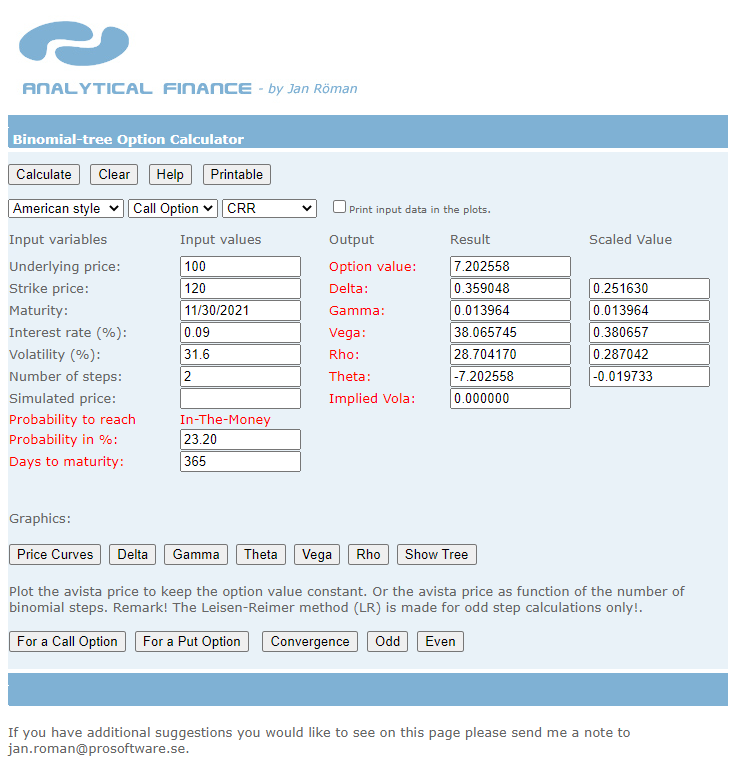
\includegraphics[scale=0.8]{Roman_binomial_calculator_inputs}
  \caption{Roman's Binomial Options Calculator Inputs}
\end{figure}

\begin{figure}[H]
  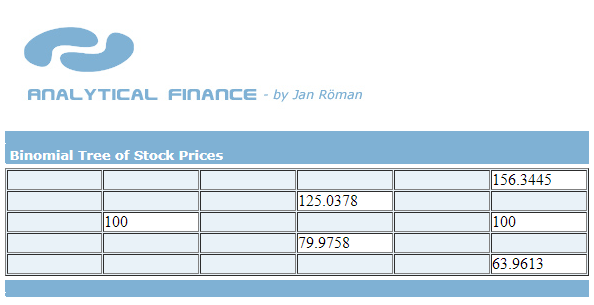
\includegraphics{Roman_binomial_calculator_stock_prices}
  \caption{Roman's Binomial Options Calculator Stock Prices}
\end{figure}

\begin{figure}[H]
  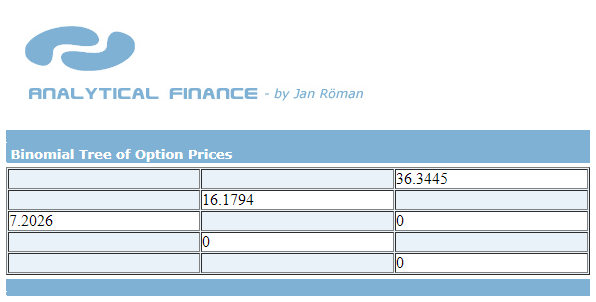
\includegraphics{Roman_binomial_calculator_option_values}
  \caption{Roman's Binomial Options Calculator Option Values}
\end{figure}

When comparing the results of Roman's calculator with the results of our example binomial tree, we can see that both stock and options values generated are very close.
The small differences of precision could be due to the rounded values, but overall, the results are near identical.

\section*{Application}
A binomial options pricing model program written in Python3 was made as the application for this project.
The program created follows and uses the methods and formulas described in this paper and can do a much larger number of steps.

The source code for this application can be found in the same repository that houses the .tex file of this PDF, accessible here:

\href{https://github.com/cliuj/binomial-options-pricing-model}{\color{blue}{https://github.com/cliuj/binomial-options-pricing-model}}

\end{document}
